\documentclass[fr]{../../../../../../eplexam}

\usepackage{titlesec, blindtext, color}
\definecolor{gray75}{gray}{0.75}

%\titleformat{\chapter}[hang]{\Huge\bfseries}{Chapitre \thechapter\hsp\textcolor{gray75}{|}\hsp}{0pt}{\Huge\bfseries}
\usepackage{lmodern}
\usepackage[T1]{fontenc}
%\usepackage{aeguill}
\usepackage[tikz]{bclogo}
\usepackage{array}
\usepackage[normalem]{ulem}
\usepackage{soul}
\usepackage{multirow}
\usepackage{sidecap}
\usepackage{xcolor}
\newcommand{\hsp}{\hspace{5mm}}
\newcommand{\tx}{\hsp \textup}
\setlist[itemize]{label=\textbullet}
\renewcommand{\r}{\textbf{r}}
\renewcommand{\k}{\textbf{k}}
 
\hypertitle{Physique des matériaux}{6}{MAPR}{1492}{2018}{Juin}{Majeure}
{Théo Gladsteen}
{L. Piraux et G-M Rignanese} 
 
\section{Partie Piraux}

\paragraph{Question 1 (2 pages)} Montrer que les impuretés jouent un rôle important dans les semiconducteurs. Décrire le cas des donneurs d'électrons. Montrer l'évolution en température de la densité d'électrons libres dans les semiconducteurs de type n.

\paragraph{Question 2 (2 pages)} Décrire les mécanismes de collisions électron-phonon dans un métal au voisinage de la température ambiante (c'est-à-dire au-dessus de la température de Debye) et en déduire la variation en température de la résistivité.

\paragraph{Question 3 (1 page max)} Déduire la variation en température de la conductivité thermique de réseau.

\paragraph{Question 4 (1/2 page)} Évaluer la variation relative de la chaleur spécifique du diamant entre 50K et 5K. En est-il de même pour le plomb ?\footnote{Suite à une question d'un étudiant, Piraux a précisé au tableau qu'il fallait s'intéresser à la différence entre le rapport $C_V(50K)/C_V(5K)$ pour le diamant et pour le plomb.}

\paragraph{Question 5 (1/2 page)} L'énergie d'un gaz d'électrons libres dans un métal simple est-elle influencée par la température ? Commentez brièvement.

\paragraph{Question 6 (1/2 page)} En quoi consiste l'anisotropie magnétique ? Illustrer succintement en considérant l'anisotropie magnétocristalline.

\paragraph{Question 7 (1/2 page)} Pour une même valeur du champ magnétique, la tension de Hall est-elle plus élevée dans un métal ou dans un semiconducteur de type n ? Justifiez brièvement votre réponse.



\newpage
\section{Partie Rignanese}
Soit une chaîne linéaire périodique d'atomes séparés les uns des autres d'une distance $L_0$. Complétez le plus précisément possible la figure ci-dessous avec la structure de bande électronique (uniquement les 4 premières bandes d'énergie $E_i(k)$ pour $i \in [1,2,3,4]$) pour les potentiels périodiques suivants : \\
\begin{enumerate}
\item $V_1(x) = 0$\\
\item $V_2(x) = 0,05 E_0 \cos (G_0 x) + 0,15 E_0 \cos (3G_0x)$\\
avec $G_0 = \frac{2\pi}{L_0}$ et $E_0 = \frac{G_0^2}{2}$ en le considérant comme un potentiel faible.
\end{enumerate}
\vspace{5mm}


Pour la facilité, les énergies $E_i(k)$ sont représentées en unités de $E_0$, c'est-à-dire que vous reportez la valeur $\frac{E_i(k)}{E_0}$, et les vecteurs d'onde $k$ sont représentés en unité de $G_0$, c'est-à-dire que vous reportez la valeur $\frac{k}{G_0}$.

\begin{center}
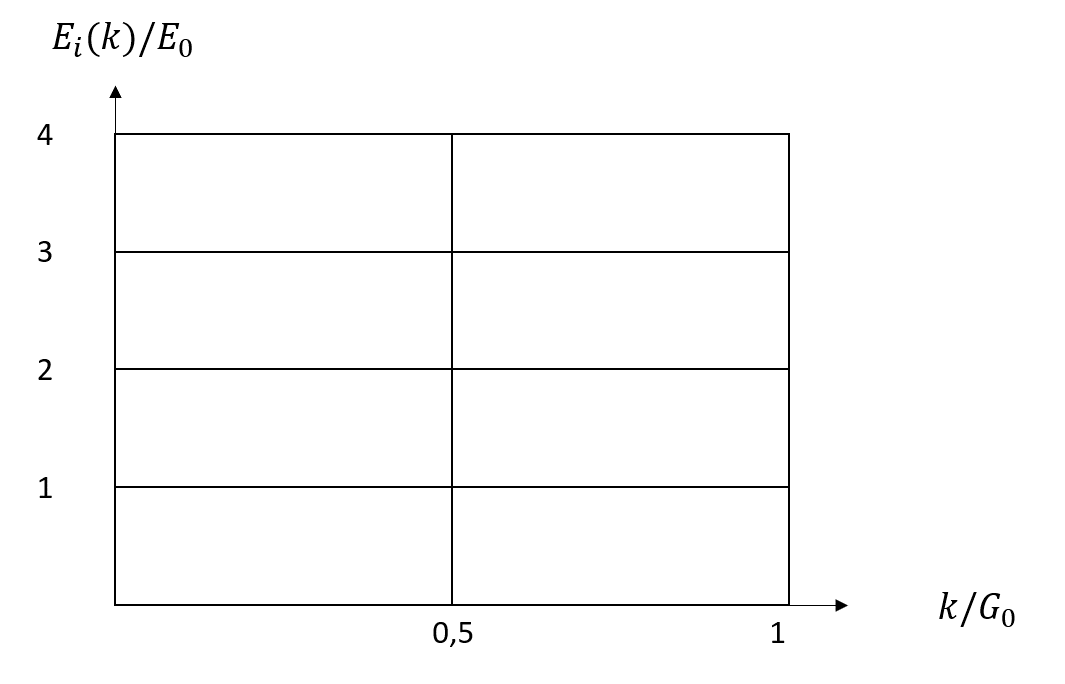
\includegraphics[width=0.7\linewidth]{juin2018M2.png}
\end{center}


Complétez également les tableaux avec les différences d'énergie. Justifiez votre dessin et les valeurs reportées.


\begin{minipage}{0.5\linewidth}
\begin{center}
\begin{tabular}{c|cccccc}
$\displaystyle V_1(x)=0$ &&& $\displaystyle\frac{k}{G_0} = 0$ &&& $\displaystyle\frac{k}{G_0} = 0,5$\\
\hline
\\
$\displaystyle\frac{E_2(k) - E_1(k)}{E_0}$ \\
\\
$\displaystyle\frac{E_3(k) - E_2(k)}{E_0}$ \\
\\
$\displaystyle\frac{E_4(k) - E_3(k)}{E_0}$ \\
\end{tabular}
\end{center}
\end{minipage}
\begin{minipage}{0.5\linewidth}
\begin{center}
\begin{tabular}{c|cccccc}
$\displaystyle V_2(x)=0$ &&& $\displaystyle\frac{k}{G_0} = 0$ &&& $\displaystyle\frac{k}{G_0} = 0,5$\\
\hline
\\
$\displaystyle\frac{E_2(k) - E_1(k)}{E_0}$ \\
\\
$\displaystyle\frac{E_3(k) - E_2(k)}{E_0}$ \\
\\
$\displaystyle\frac{E_4(k) - E_3(k)}{E_0}$ \\
\end{tabular}
\end{center}
\end{minipage}

\end{document}
